\chapter{Solução Proposta}
\label{chap:Chapter4}
Neste capítulo apresenta-se a abordagem conceptualizada e implementada no protótipo. Na Secção~\ref{sec:chap04_general_vision} descreve-se a solução na sua globalidade, dando ênfase à arquitetura de sistema e à descrição de cada componente. Posteriormente, na Secção~\ref{sec:chap04_conception}, descrevem-se os aspetos relevantes da conceção, incluindo o processo de trabalho usado ao longo desta fase, os requisitos identificados, a análise e desenho do sistema. Na Secção~\ref{sec:chap04_development} expõem-se os pormenores de desenvolvimento do protótipo considerados relevantes e, por fim, na Secção~\ref{sec:chap04_validation} apresentam-se os tópicos de validação, cujos resultados obtidos serão pertinentes para a conclusão da presente tese.

\section{Visão Geral} 
\label{sec:chap04_general_vision}

\begin{sidewaysfigure}
    \centering
    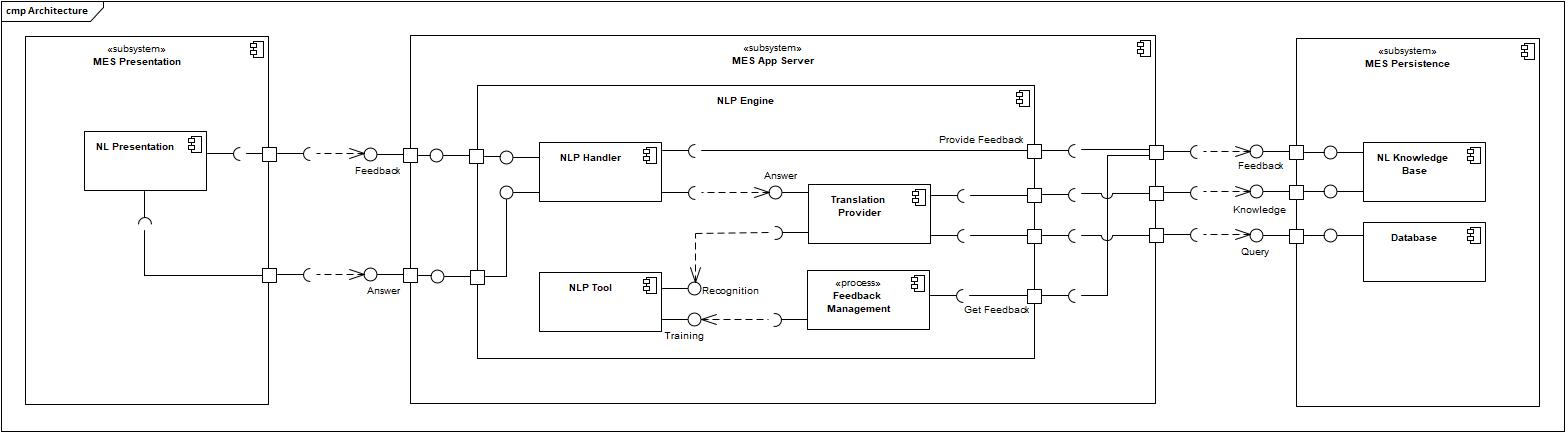
\includegraphics[width=\textwidth]{ch04/assets/Architecture.jpg}
    \caption{Arquitetura do protótipo}
    \label{fig:prototype_architecture}
\end{sidewaysfigure}

\tbd

\section{Conceção} 
\label{sec:chap04_conception}
\tbd

\section{Desenvolvimento} 
\label{sec:chap04_development}
\tbd

\section{Validação} 
\label{sec:chap04_validation}
\tbd
